\section{Results \& Discussion}

\subsection{Ablation Study: The Critical Role of Spectral Normalization}
In Phase 1 of our experimental pipeline, we systematically investigated the impact of Spectral Normalization (SN) on the SV-DKL architecture to empirically validate the feature collapse hypothesis. Table \ref{tab:spectral_norm} presents the aggregated Test set metrics for the top-5 performing Optuna trials of both the unconstrained and the spectrally normalized models. 

\begin{table}[h]
\centering
\caption{Test Metrics across top-5 SV-DKL Optuna runs (Mean $\pm$ Std. Dev.)}
\label{tab:spectral_norm}
\begin{tabular}{@{}lccc@{}}
\toprule
Metric & SV-DKL (No Spectral Norm) & SV-DKL (With Spectral Norm) & Difference ($\Delta$) \\ \midrule
MAE $\downarrow$ & 0.404 $\pm$ 0.027 & \textbf{0.380 $\pm$ 0.015} & -0.024 \\
NLL $\downarrow$ & 0.753 $\pm$ 0.086 & \textbf{0.663 $\pm$ 0.021} & -0.090 \\
AURC $\downarrow$ & 0.369 $\pm$ 0.019 & \textbf{0.327 $\pm$ 0.022} & -0.042 \\
PICP\_95 $\uparrow$ & 0.915 $\pm$ 0.028 & \textbf{0.970 $\pm$ 0.008} & +0.055 \\ \bottomrule
\end{tabular}
\end{table}

The unregularized models failed fundamentally across all probabilistic and predictive dimensions on the unseen Test set. Notably, while the unconstrained networks often achieved slightly lower \textit{validation} MAE during early stopping (an artifact of the MLP aggressively warping the latent space to overfit the validation manifold), this mapping generalized poorly to novel molecules, resulting in a higher Test MAE (0.404 vs 0.380).

More critically, the probabilistic metrics reveal severe OOD blindness. The application of the bi-Lipschitz constraint via Spectral Normalization drove the NLL down by 0.090 and restored the 95\% Prediction Interval Coverage Probability (PICP\_95) from a degraded 91.5\% to a highly calibrated 97.0\%. 

This qualitative difference is starkly visualized in the Rejection Curves (Figure \ref{fig:rejection_curve}). Without SN, the Rejection Curve is largely flat. Mathematically, this implies that the model's predicted variance ($\sigma^*$) is entirely orthogonal to its actual residual error ($|y - \mu^*|$); discarding the "most uncertain" predictions does not meaningfully improve the error rate of the retained subset. With SN, the curve decays monotonically, confirming that the Lipschitz constraint successfully preserves input-space distances. The GP correctly identifies and assigns high epistemic uncertainty to the hardest OOD molecules, driving the AURC down to 0.327.

\begin{figure}[h]
    \centering
    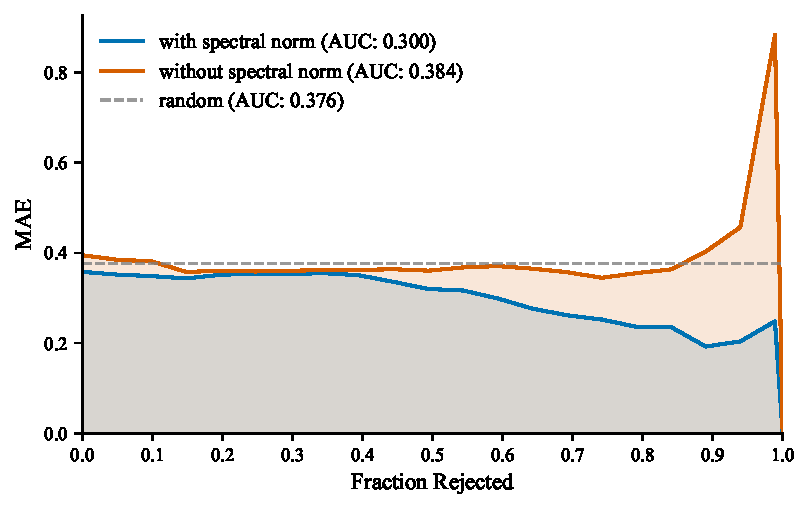
\includegraphics[width=0.7\linewidth]{figures/spectral-norm-rc-comparison.pdf}
    \caption{Test Set Rejection Curves. A flat curve (No SN) indicates feature collapse, where estimated uncertainty fails to correlate with true error. Spectral Normalization restores distance awareness, allowing the model to accurately rank its epistemic uncertainty and driving the AURC downward.}
    \label{fig:rejection_curve}
\end{figure}

\subsection{SV-DKL vs. XGBoost: Overcoming the Geometric Mismatch}
In Phase 2, we benchmarked our optimal SV-DKL model against a classical XGBoost Deep Ensemble. Despite an exhaustive 200-trial hyperparameter sweep pushing tree parameters to their theoretical limits of regularization (e.g., highly constrained tree depth, massive estimator counts, and aggressive feature subsampling to combat the $P \gg N$ regime), the optimal XGBoost model failed to match the fully tuned SV-DKL architecture.

\begin{table}[h]
\centering
\caption{Test Metrics Evaluation: Best XGBoost Deep Ensemble vs. Best SV-DKL Model}
\label{tab:model_comparison}
\begin{tabular}{@{}lcc@{}}
\toprule
Metric & XGBoost Deep Ensemble & SV-DKL (With Spectral Norm) \\ \midrule
MAE $\downarrow$ & 0.373 & \textbf{0.358} \\
NLL $\downarrow$ & 39.627 & \textbf{0.652} \\
PICP\_95 $\uparrow$ & 0.209 & \textbf{0.984} \\
AURC $\downarrow$ & 0.357 & \textbf{0.299} \\ \bottomrule
\end{tabular}
\end{table}

The probabilistic failure of the XGBoost ensemble is absolute. An NLL of 39.627 and a collapsed coverage probability of 20.9\% (PICP\_95) highlights the architecture's inability to quantify continuous uncertainty in low-data regimes. Because the $N \approx 582$ training set is so sparse, the independent members of the ensemble ultimately converge on very similar axis-aligned splits. This lack of architectural diversity results in pathologically narrow predictive intervals (variance collapse). When the ensemble inevitably makes an error with a near-zero predicted variance, the Gaussian NLL penalty explodes exponentially, rendering the model a "confident fool."

Furthermore, the point accuracy gap (MAE of 0.373 vs 0.358) exposes a fundamental \textit{Geometric Mismatch}. Decision trees rely on orthogonal, axis-aligned hyper-rectangular partitions. When forced to segment the continuous, highly distributed latent space of a MoLFormer embedding, trees must build highly inefficient, jagged approximations of smooth decision boundaries. If the trees are allowed to grow deep enough to approximate these curves, they instantly memorize the tiny training set. If they are constrained to prevent overfitting (as enforced by our Optuna sweep), they underfit the underlying molecular relationships. 

Conversely, the SV-DKL natively utilizes spatial covariance metrics (via the GP Kernel) across the entire 768-dimensional vector simultaneously. By evaluating holistic Euclidean or Mahalanobis distances rather than slicing individual axes, SV-DKL naturally exploits the foundation model's dense geometry exactly as it was designed to be interpreted.

\begin{figure}[h]
    \centering
    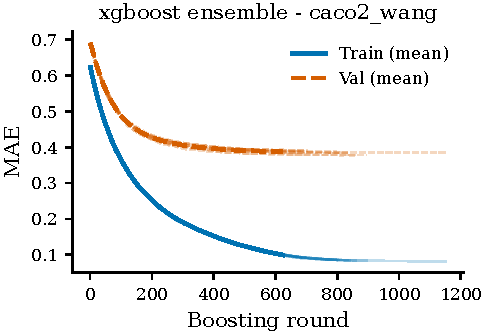
\includegraphics[width=0.5\linewidth]{figures/ensemble-training-curves.pdf}
    \caption{Training vs. Validation MAE per epoch for the XGBoost ensemble. The plot illustrates the struggle with the geometric mismatch: tree-based models rapidly memorize the small $N$ training set, while generalization on the validation set severely plateaus despite extreme regularization.}
    \label{fig:training_curves}
\end{figure}